%versi 3 (22-07-2020)
\chapter{Landasan Teori}
\label{chap:landasan_teori}

\section{Point of Interest}
\label{sec:poi}

\textit{Point of Interest} (POI) adalah sebuah lokasi geografis yang memiliki kegunaan tertentu. POI biasanya dikenali oleh banyak orang dan memiliki keunikan tertentu pada tampilannya. Salah satu contoh POI dapat dilihat pada Gambar~\ref{fig:poi}. POI juga dapat dimanfaatkan untuk menjadi penanda lokasi seseorang. Seseorang dapat mengerti lokasinya dengan melihat POI yang ada di sekitarnya.
\begin{figure}[H]
	\centering
	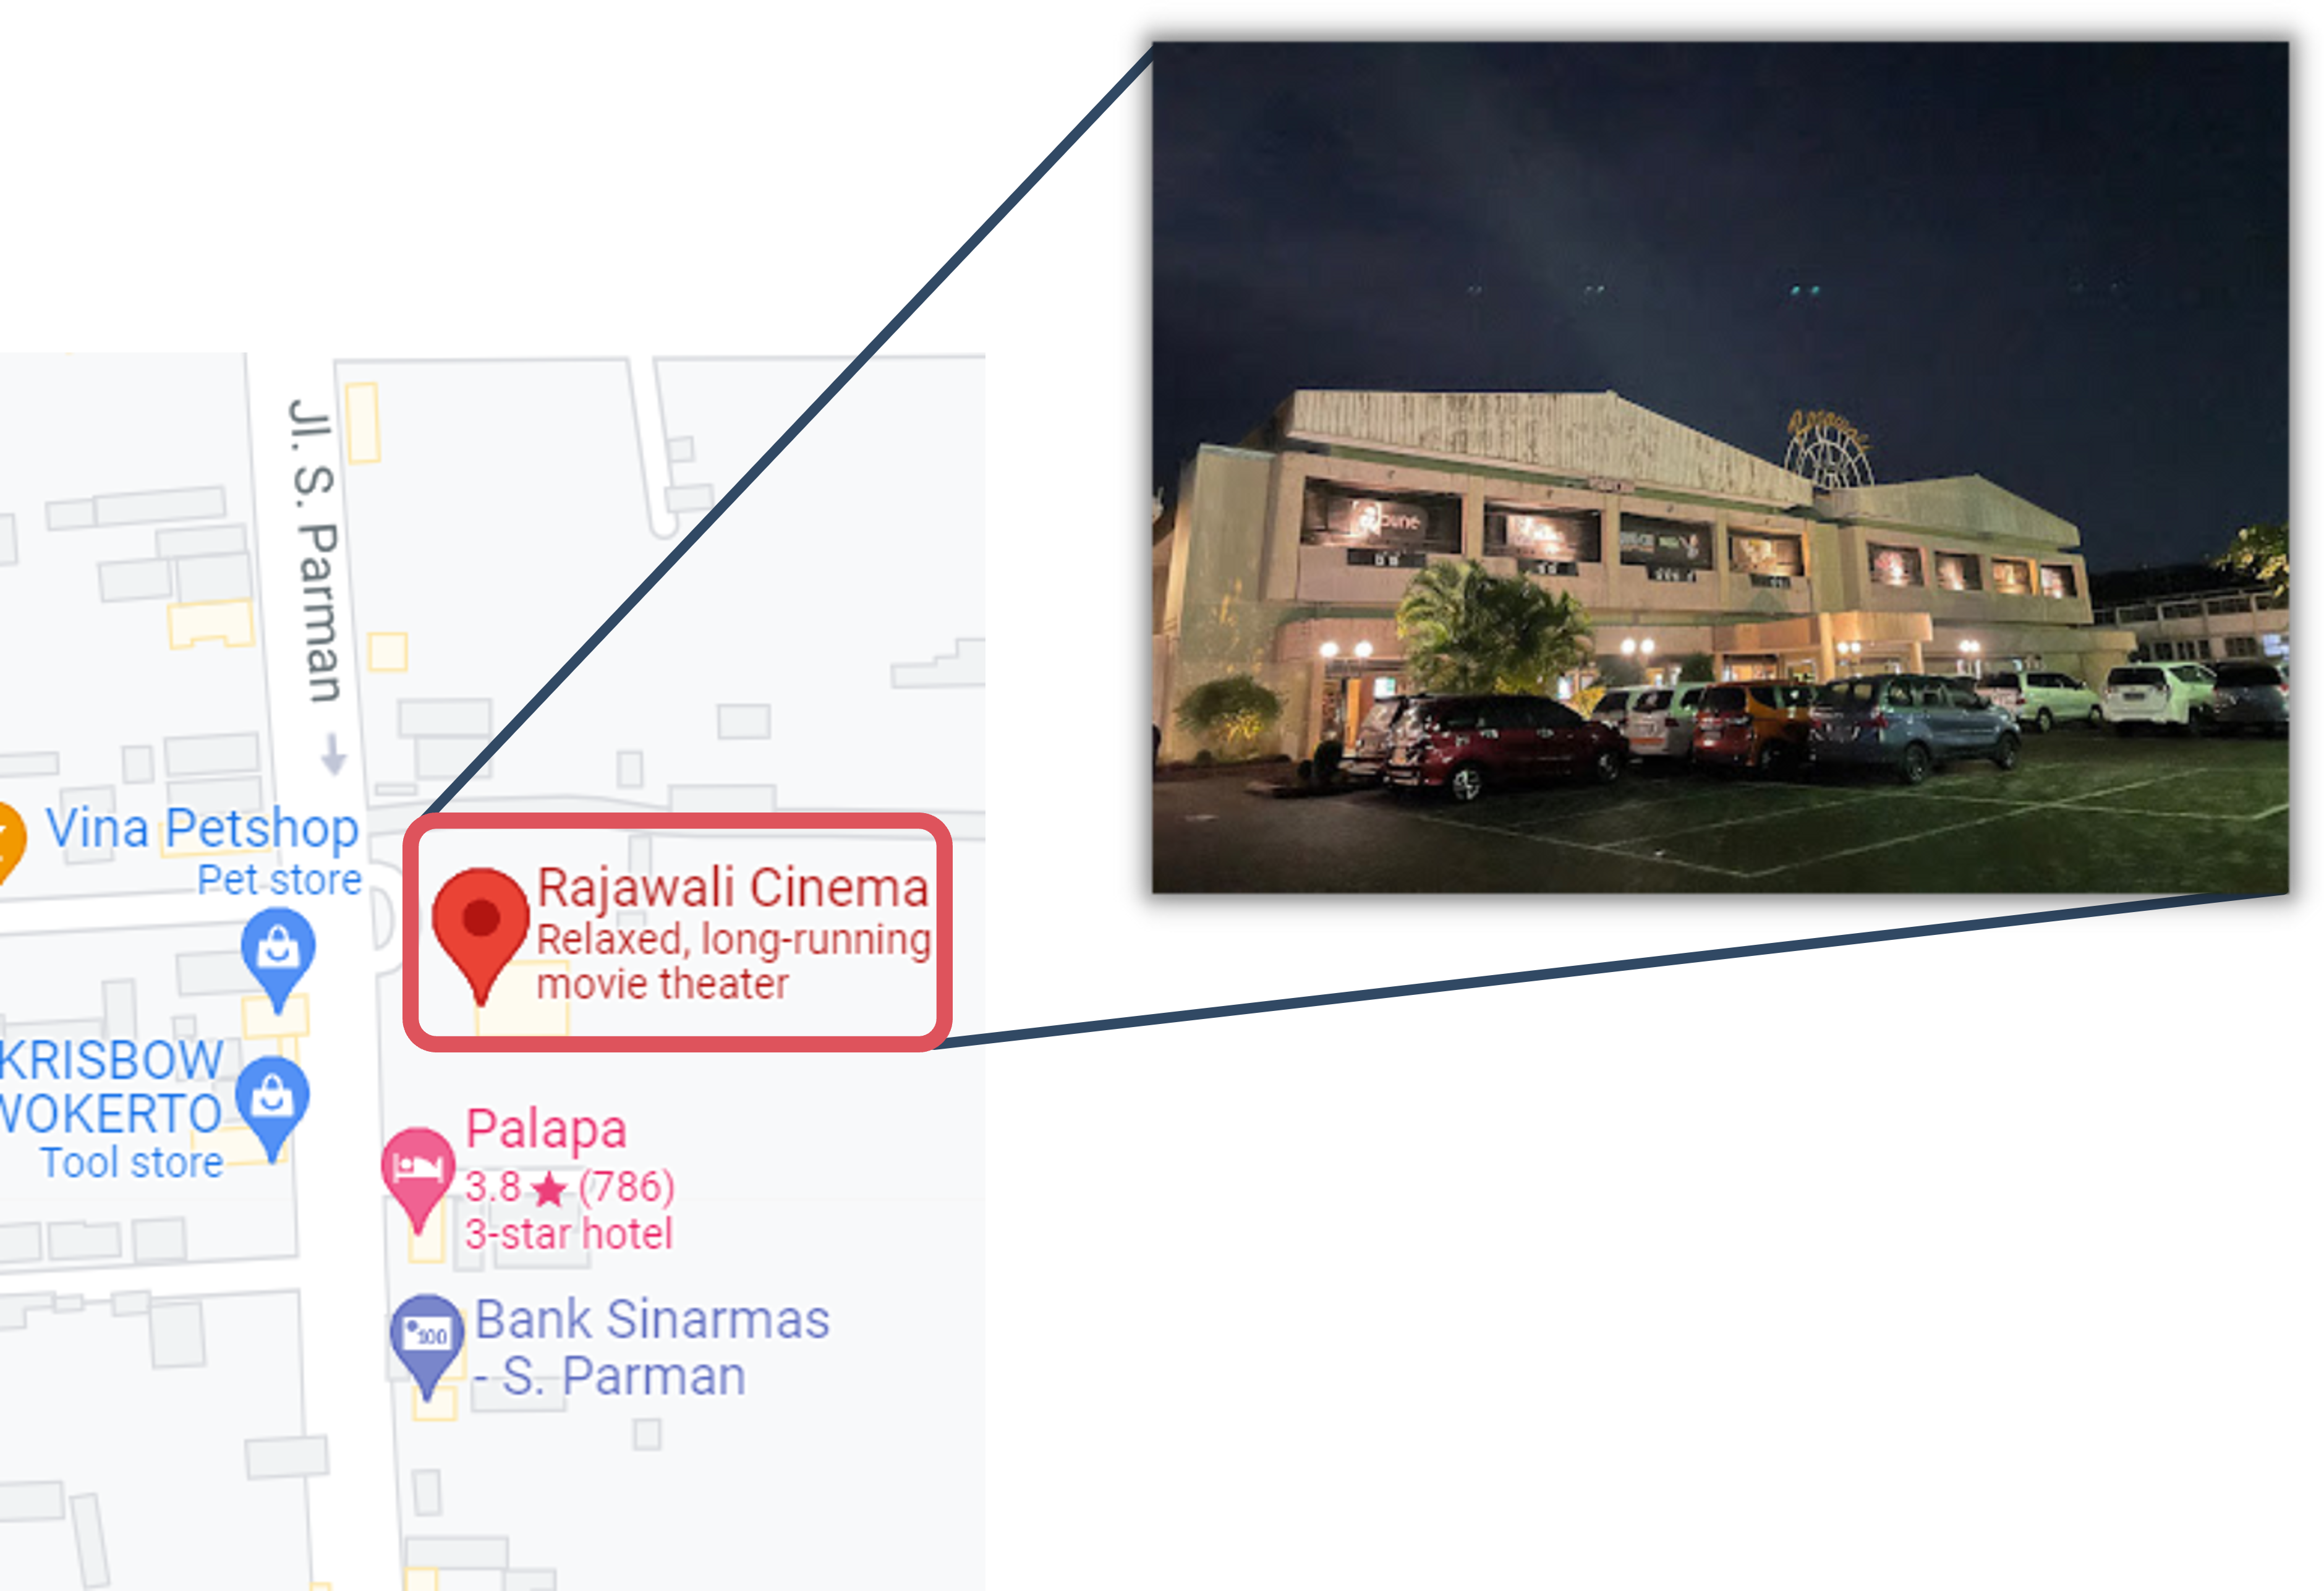
\includegraphics[width=0.6\linewidth]{poi.png}
	\caption{Salah satu contoh POI.}
	\label{fig:poi}
\end{figure}

Beberapa POI tertentu dapat memiliki logo yang sifatnya unik. POI tersebut dapat dikenali dengan hanya melihat logonya saja. Contoh bisa dilihat pada Gambar~\ref{fig:poi_logo}. POI dengan logo unik ini dapat dikenali oleh komputer salah satunya dengan menggunakan teknik \textit{Object Instance Recognition} (OIR). 
\begin{figure}[H]
	\centering
	\includegraphics[width=0.35\linewidth]{kfc_circled.png}
	\includegraphics[width=0.35\linewidth]{hnm_circled.png}
	\caption{Contoh POI dengan logo unik.}
	\label{fig:poi_logo}
\end{figure}

\section{Object Instance Recognition}
\label{sec:oir}

\textit{Object Instance Recognition} (OIR) adalah teknik pengenalan objek spesifik. Pada teknik OIR deteksi tidak memberikan kelas dari gambar tetapi label yang khusus, seperti contohnya jika objek merupakan sebuah mobil, OIR akan memberikan jenis model mobil tersebut. OIR bekerja dengan menerima gambar masukkan dan mencari gambar pada \textit{dataset} yang memiliki paling banyak kemiripan.

OIR dapat dilakukan dengan menggunakan fitur lokal. Fitur lokal sendiri merupakan fitur dalam gambar yang mendeskripsikan sebuah daerah tertentu pada gambar tersebut. Fitur lokal dapat berupa perpotongan garis atau yang biasa disebut \textit{keypoint}. Sebuah \textit{keypoint} akan dapat diidentifikasi dengan menggunakan daerah di sekitar \textit{keypoint} tersebut. Deskripsi \textit{keypoint} ini dibuat dalam sebuah vektor yang dinamakan vektor deskriptor.

Teknik OIR bekerja dengan melakukan deteksi fitur lokal pada gambar masukkan dan pada gambar-gambar di \textit{dataset}. Fitur-fitur lokal dari gambar masukkan tersebut kemudian dipasangkan dengan fitur lokal dari gambar \textit{dataset}. Gambar yang memiliki pasangan terbanyak akan merupakan hasil deteksi gambar masukkan tersebut. 

Masalah OIR akan mudah bila gambar masukkan merupakan gambar yang sudah bersih. Pada praktiknya sebuah algoritma OIR seharusnya tetap dapat mengenali objek walaupun gambar bervariasi. Beberapa perubahan pada gambar berikut merupakan faktor-faktor yang dapat mempersulit proses OIR:
\begin{itemize}
	\item Cahaya \\
	Perubahan pada tingkat pencahayaan pada gambar yang mengakibatkan perubahan nilai \textit{pixel-pixel} pada gambar.
	\item Skala \\
	Jarak diambilnya gambar yang berisi objek. Perbedaan ukuran objek pada gambar akan menyebabkan sudut-sudut pada objek menjadi berbeda.
	\item Rotasi \\
	Orientasi atau arah pengambilan gambar yang berbeda akan mengakibatkan objek pada gambar jadi terlihat berbeda. Sudut-sudut akan menjadi berbeda karena arah hadapnya berbeda.
	\item Latar Belakang \\
	Objek-objek lain di sekitar objek yang ingin diidentifikasi akan berpotensi mempersulit pemrosesan. Objek-objek tersebut dapat menghasilkan fitur-fitur lokal yang tidak relevan terhadap objek yang ingin diidentifikasi.
	\item Bagian Objek Tertutup \\
	Adanya objek lain yang menutupi sebagian dari objek yang ingin diidentifikasi akan berpotensi menyebabkan beberapa fitur lokal dari objek tidak terdeteksi.
	\item Sudut Pandang \\
	Sudut pengambilan gambar yang berbeda akan memengaruhi pemrosesan. Fitur-fitur lokal dari objek yang ingin diidentifikasi akan menjadi berbeda.
	\item Translasi \\
	Posisi objek yang ingin diidentifikasi dalam gambar akan memengaruhi pemrosesan. Pencarian pasangan fitur lokal tidak dapat dengan hanya menggunakan posisi di mana fitur lokal tersebut ditemukan pada gambar.
\end{itemize}

Pengambilan fitur lokal dari gambar dapat dilakukan dengan beberapa metode, seperti SIFT (lihat~\ref{sec:sift}) dan ORB (lihat~\ref{sec:orb}). Kedua metode tersebut---SIFT dan ORB---sudah menangani masalah perubahan skala dan rotasi karena fitur lokal yang dihasilkan oleh SIFT dan ORB bersifat invarian terhadap skala dan rotasi.

Proses pencarian pasangan fitur lokal dari gambar masukkan dan \textit{dataset} dilakukan dengan menggunakan vektor deskriptor dari fitur lokal. Perubahan-perubahan pada gambar walaupun sedikit akan menyebabkan perubahan nilai pada vektor deskriptor. Vektor deskriptor dari fitur lokal pada gambar masukkan hampir tidak akan persis sama dengan vektor deskriptor dari gambar yang ada di \textit{dataset}. Oleh karena itu pencarian pasangan fitur lokal dilakukan dengan mencari pasangan fitur lokal yang memiliki nilai kemiripan paling tinggi.

Secara garis besar tahapan proses OIR pada penelitian ini adalah sebagai berikut:
\begin{enumerate}
	\item Ekstraksi Fitur \\
	Pertama akan dilakukan pengambilan fitur-fitur lokal dari gambar masukkan. Dengan menggunakan metode SIFT atau ORB pengambilan fitur lokal akan menghasilkan \textit{list} yang  berisi \textit{keypoint}. Setiap \textit{keypoint} yang dihasilkan akan memiliki sebuah vektor yang akan digunakan untuk mengidentifikasi \textit{keypoint} tersebut.
	\item Pairing \\
	Untuk setiap fitur lokal yang terdeteksi pada gambar masukkan akan dicari beberapa fitur lokal dari gambar pada \textit{dataset} yang paling mirip. Kemiripan fitur lokal ditentukan dengan menghitung jarak \textit{Euclidean} antara vektor deskriptor kedua fitur lokal tersebut.
	\item Verification \\
	Pasangan fitur lokal yang didapat pada tahap sebelumnya merupakan pasangan yang hanya memiliki ciri yang mirip tetapi belum tentu konsisten secara geometris. Pasangan fitur lokal dikatakan konsisten secara geometris jika keduanya memiliki posisi yang sama relatif terhadap objek di sekitarnya. Ilustrasi dapat dilihat pada Gambar~\ref{fig:geo_ver}. Hanya pasangan-pasangan fitur lokal yang konsisten secara geometris yang akan diproses lebih lanjut.
	\item Scoring \\
	Setelah didapatkan semua pasangan fitur lokal yang paling mirip dan konsisten secara geometris maka dapat ditentukan pasangan gambar yang menjadi label gambar masukkan. Kemudian perlu dihitung nilai kemiripan dari label yang dihasilkan. Kemiripan dapat dihitung dengan menghitung $\frac{1}{d}$ untuk semua pasangan fitur lokal, di mana $d$ merupakan jarak \textit{Euclidean} pasangan tersebut. Nilai-nilai $\frac{1}{d}$ tersebut kemudian dihitung totalnya untuk menjadi nilai kemiripan label hasil.
	
\end{enumerate}
\begin{figure}[H]
	\begin{subfigure}[b]{.5\textwidth}
		\centering
		\includegraphics[width=0.9\linewidth]{geo_ver1.png}
		\caption{}
		\label{subfig:geo_ver1}
	\end{subfigure}%
	\begin{subfigure}[b]{.5\textwidth}
		\centering
		\includegraphics[width=0.9\linewidth]{geo_ver2.png}
		\caption{}
		\label{subfig:geo_ver2}
	\end{subfigure}
	\caption{Ilustrasi fitur lokal yang konsisten dan tidak konsisten. Pasangan fitur lokal A1 dengan A2 konsisten secara geometris karena keduanya memiliki posisi yang sama relatif terhadap fitur lokal lain. Fitur lokal A1 berada di atas B1 dan C1 sedangkan fitur lokal A2 berada di atas B2 dan C2. Pasangan fitur lokal B1 dengan B2 dan C1 dengan C2 tidak konsisten secara geometris karena B1 berada di kanan C1 sedangkan B2 berada di sebelah kiri C2.}
	\label{fig:geo_ver}
\end{figure}

\section{SIFT (Speeded Up Robust Feature)}
\label{sec:sift}

SIFT adalah salah satu metode pencarian fitur lokal yang dicetuskan pada~\cite{lowe2004sift}. Fitur lokal yang dihasilkan SIFT bersifat invarian terhadap rotasi, perubahan skala, dan translasi pada gambar. Sifat invarian ini berarti fitur lokal yang sama pada gambar yang telah di rotasi, diubah skalanya, atau di translasi akan tetap memiliki ciri yang mirip. Setiap fitur lokal akan memiliki sebuah vektor yang mendeskripsikan daerah area fitur lokal tersebut, vektor ini biasa disebut sebagai deskriptor. Vektor deksriptor SIFT berbentuk vektor bilangan bulat yang memiliki 128 elemen. Tahap pencarian fitur lokal pada SIFT dibagi menjadi 4 langkah sebagai berikut.

\subsection{Pencarian Extrema}
Pada tahap ini akan dicari \textit{pixel-pixel} pada gambar yang merupakan \textit{corner} atau biasa disebut \textit{keypoint}. \textit{Keypoint} pada SIFT dicari dengan memeriksa \textit{pixel-pixel} pada gambar hasil turunan kedua Gaussian. Turunan kedua Gaussian akan dihitung dengan menggunakan \textit{Difference of Gaussian} (DoG).

Penghitungan DoG ini dilakukan dengan memanfaatkan sifat dari \textit{Matrix} Konvolusi Gaussian. \textit{Matrix} Konvolusi Gaussian merupakan \textit{matrix} yang memiliki sifat distribusi Gaussian, di mana titik tengah \textit{matrix} memiliki nilai yang tinggi dan nilai-nilai di sekitarnya berkurang semakin mendekati tepi \textit{matrix}. Seperti ditunjukkan pada Gambar~\ref{fig:gaussian_function}. 
\begin{figure}[H]
	\begin{subfigure}[b]{.5\textwidth}
		\centering
		\includegraphics[width=1\linewidth]{gaussian_curve_s.png}
		\caption{}
		\label{subfig:gaussian_curve}
	\end{subfigure}%
	\begin{subfigure}[b]{.5\textwidth}
		\centering
		\includegraphics[width=0.9\linewidth]{gaussian_matrix_3.png}
		\caption{}
		\label{subfig:gaussian_matrix}
	\end{subfigure}
	\caption{Kurva Gaussian dan bentuk representasi \textit{matrix}-nya.}
	\label{fig:gaussian_function}
\end{figure}

Pada fungsi Gaussian tingkat penyebaran data dapat diatur dengan mengubah parameter $\sigma$ yang mengatur nilai standar deviasi. Gambar~\ref{subfig:gaussian_curve} menunjukkan bagaimana nilai $\sigma$ mengatur bagaimana data tersebar dari \textit{mean}, di mana semakin tinggi nilai $\sigma$ maka data akan semakin menyebar. Nilai yang semakin menyebar menyebabkan perbedaan nilai antar titik semakin kecil. Efeknya pada \textit{matrix} dapat dilihat pada Gambar~\ref{fig:gaussian_sigma}. Nilai $\sigma$ yang tinggi menyebabkan kurva semakin melebar dan pada \textit{matrix} selisih nilai antar titik menjadi semakin kecil.

\begin{figure}[H]
	\begin{subfigure}[b]{.5\textwidth}
		\centering
		\includegraphics[width=0.9\linewidth]{gaussian_curve_1.png}
		\includegraphics[width=0.9\linewidth]{gaussian_matrix_1.png}
		\caption{$\sigma=1$}
		\label{subfig:gaussian_sigma1}
	\end{subfigure}%
	\begin{subfigure}[b]{.5\textwidth}
		\centering
		\includegraphics[width=0.9\linewidth]{gaussian_curve_2.png}
		\includegraphics[width=0.9\linewidth]{gaussian_matrix_2.png}
		\caption{$\sigma=2$}
		\label{subfig:gaussian_sigma2}
	\end{subfigure}
	\caption{Kurva dan \textit{matrix} Gaussian pada nilai $\sigma$ yang berbeda.}
	\label{fig:gaussian_sigma}
\end{figure}

\textit{Matrix} Konvolusi Gaussian ketika diaplikasikan pada gambar akan menyebabkan perubahan nilai tiap \textit{pixel} pada gambar. Nilai dari setiap \textit{pixel} akan menjadi mirip dengan \textit{pixel} tetangga di dekatnya. Perubahan nilai \textit{pixel} akan paling berpengaruh pada daerah dengan perubahan nilai \textit{pixel} yang tinggi. Tingkat perubahan nilai dipengaruhi oleh nilai $\sigma$ yang digunakan, nilai $\sigma$ yang tinggi akan menyebabkan nilai \textit{pixel} yang berdekatan semakin mirip---perubahan nilai \textit{pixel} pada daerah tersebut semakin mengecil. Jika dilihat pada gambar, maka gambar hasil konvolusi akan terlihat kabur (\textit{blur}). Nilai $\sigma$ menentukan tingkat \textit{blur} gambar.

\begin{figure}[H]
	\centering
	\begin{subfigure}[b]{.33\textwidth}
		\centering
		\includegraphics[width=0.9\linewidth]{1.0_asus_logo2.jpeg}
		\caption{$\sigma=1.0$}
		\label{subfig:asus_sigma1.0}
	\end{subfigure}%
	\begin{subfigure}[b]{.33\textwidth}
		\centering
		\includegraphics[width=0.9\linewidth]{1.4_asus_logo2.jpeg}
		\caption{$\sigma=1.4$}
		\label{subfig:asus_sigma1.4}
	\end{subfigure}
	\begin{subfigure}[b]{.33\textwidth}
		\centering
		\includegraphics[width=0.9\linewidth]{1.8_asus_logo2.jpeg}
		\caption{$\sigma=1.8$}
		\label{subfig:asus_sigma1.8}
	\end{subfigure}
	\caption{Efek nilai $\sigma$ pada hasil gambar konvolusi.}
	\label{fig:asus_konv}
\end{figure}

Perubahan nilai $\sigma$ pada \textit{matrix} konvolusi serta efeknya pada gambar akan dimanfaatkan untuk menghitung \textit{Difference of Gaussian} (DoG). DoG merupakan hasil turunan kedua Gaussian pada gambar. Gambar DoG dapat diperoleh dengan menghitung perbedaan nilai tiap \textit{pixel} dari dua gambar yang telah dikonvolusi oleh \textit{matrix} Gaussian dengan nilai $\sigma$ yang berbeda. Perbedaan nilai untuk DoG dihitung dengan mengurangi setiap \textit{pixel} pada gambar konvolusi yang memiliki nilai $\sigma$ yang lebih kecil, dengan setiap \textit{pixel} pada posisi yang sama pada gambar konvolusi yang memiliki nilai $\sigma$ yang lebih besar. Ilustrasi dapat dilihat pada Gambar~\ref{fig:dog_asus}. 
\begin{figure}[H]
	\centering
	
\includegraphics[width=\linewidth]{asus_dog.png}
	\caption{Operasi DoG pada gambar}
	\label{fig:dog_asus}
\end{figure} 

Metode SIFT mencari \textit{keypoint} dengan memanfaatkan konsep DoG. Sebuah gambar akan dikonvolusi dengan \textit{matrix} Gaussian beberapa kali dengan nilai $\sigma$ yang berbeda. Setelah didapatkan beberapa gambar maka akan dihitung DoG untuk setiap gambar yang nilai $\sigma$-nya bersebelahan (Gambar~\ref{fig:dog_scales}). Pasangan gambar konvolusi yang berbeda akan menghasilkan gambar DoG yang berbeda juga.  

Untuk setiap gambar DoG akan ditentukan \textit{pixel} mana saja yang merupakan \textit{keypoint} dengan mencari \textit{pixel} yang merupakan \textit{extrema}. Sebuah \textit{pixel} merupakan \textit{extrema} jika nilai pixel tersebut lebih besar dari seluruh 26 \textit{pixel} di sekitarnya atau lebih kecil dari seluruhnya. Ke-26 \textit{pixel} tersebut merupakan 8 \textit{pixel} yang mengelilingi, 9 \textit{pixel} pada posisi yang sama dari gambar di atasnya, dan juga 9 \textit{pixel} pada posisi yang sama dari gambar di bawahnya.
\begin{figure}[H]
	\centering
	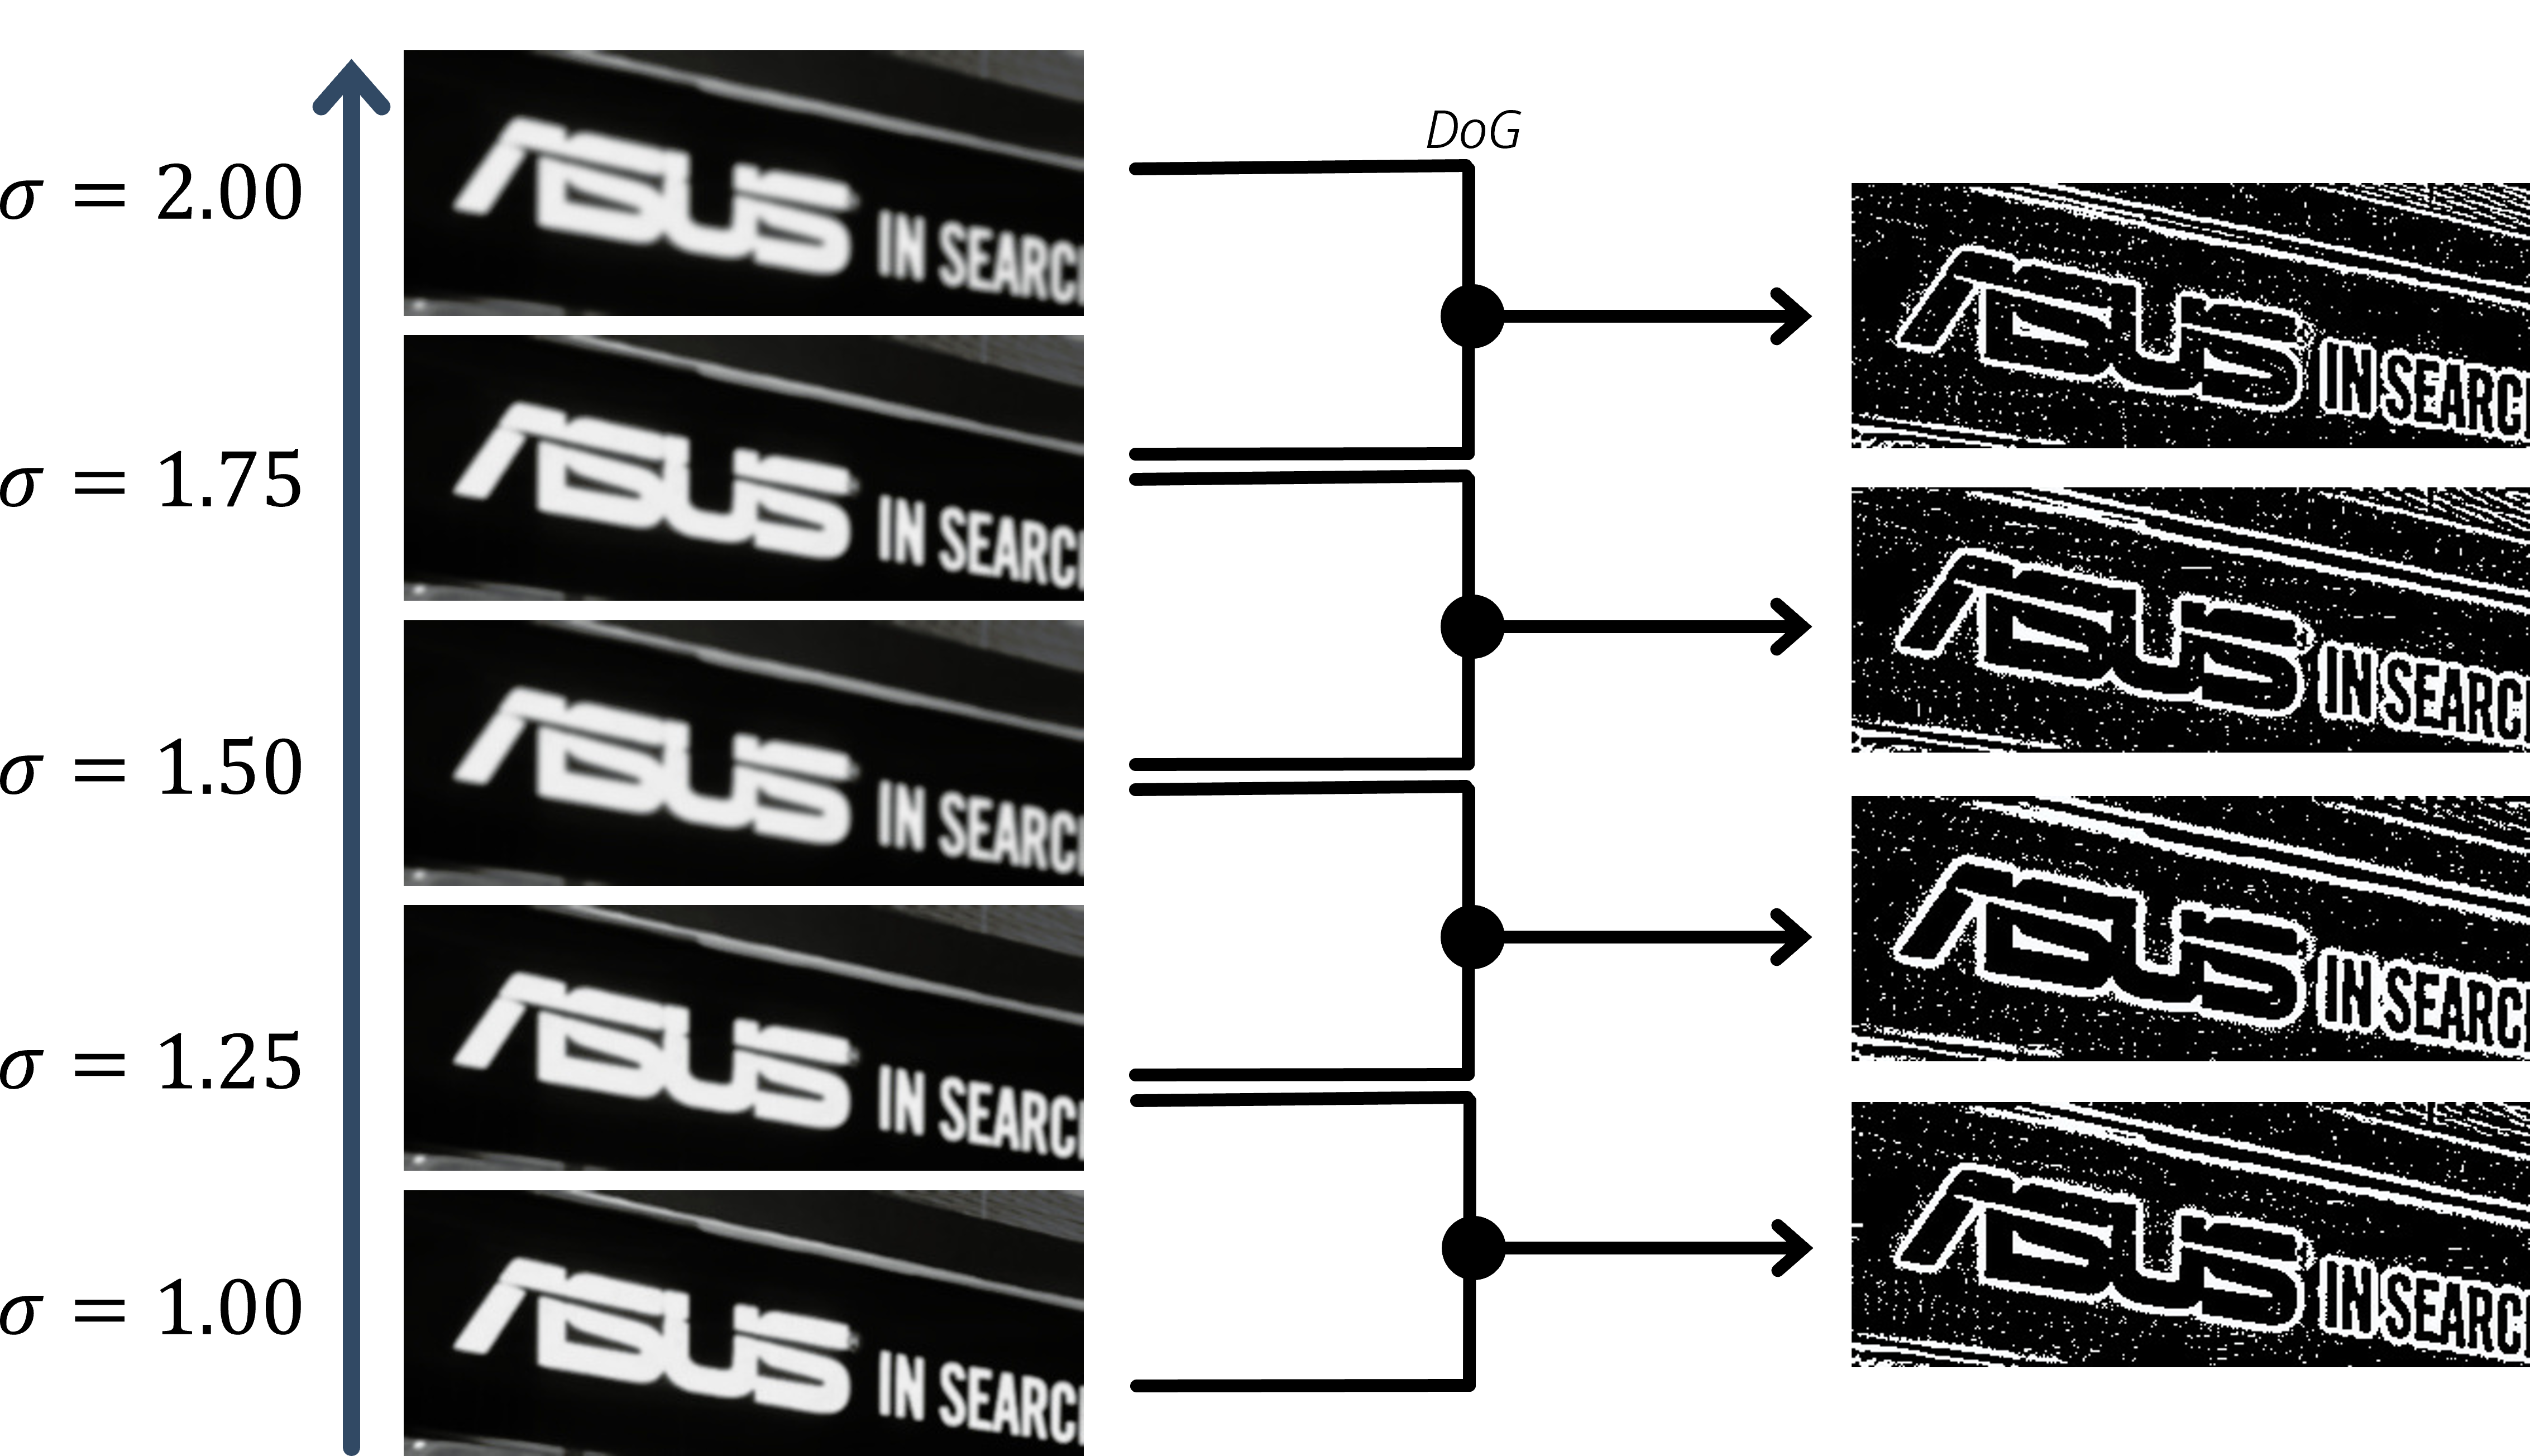
\includegraphics[width=0.7\linewidth]{dog_scales.png}
	\caption{Penggunaan DoG pada SIFT}
	\label{fig:dog_scales}
\end{figure} 

\subsection{Penentuan Skala}
Pada tahap sebelumnya sudah didapatkan \textit{keypoint-keypoint} dalam gambar. Agar \textit{keypoint} dapat invarian terhadap skala, \textit{keypoint} perlu untuk dapat tetap terdeteksi walaupun ukuran gambar berubah. Untuk setiap \textit{keypoint} perlu untuk dicari skala terkecil di mana \textit{keypoint} tersebut dapat terdeteksi. Untuk mencapai ini SIFT menggunakan lanjutan dari metode pada Gambar~\ref{fig:dog_scales} dengan langkah sebagai berikut (ilustrasi pada Gambar~\ref{fig:oktaf}):
\begin{enumerate}
	\item Lakukan konvolusi sampai nilai $\sigma$ sudah mencapai 2 kali nilai awal
	\item Perkecil ukuran gambar (\textit{downsample}) menjadi setengahnya
	\item Kembalikan nilai $\sigma$ ke nilai awal
	\item Ulang tahap dari langkah 1 hingga gambar sudah terlalu kecil.
\end{enumerate}

Pada langkah di atas setiap siklus ukuran gambar disebut sebagai oktaf, dimulai dari oktaf pertama, lalu kedua, dan seterusnya. Dengan setiap oktaf ukuran gambar akan semakin kecil. Pencarian \textit{keypoint} dilakukan pada tiap oktaf, dan untuk tiap \textit{keypoint} tersebut ditulis nilai oktaf tertinggi (ukuran gambar terkecil) di mana \textit{keypoint} tersebut dapat terdeteksi.

\begin{comment}
Saat nilai $\sigma$ sudah mencapai 2 kali dari nilai awalnya---atau yang disebut sudah menyelesaikan satu oktaf---maka proses akan dilanjutkan ke oktaf berikutnya, gambar akan diperkecil (\textit{downsample}) ukuran menjadi setengahnya dan proses konvolusi diulang lagi (Gambar~\ref{fig:oktaf}). Untuk oktaf baru tersebut akan dihitung DoG-nya dan dicari \textit{extrema}-nya. Untuk setiap \textit{keypoint} akan dicatat oktaf terbesar (ukuran gambar terkecil) di mana gambar \textit{keypoint} tersebut tetap ditemukan. 
\end{comment}

\begin{figure}[H]
	\centering
	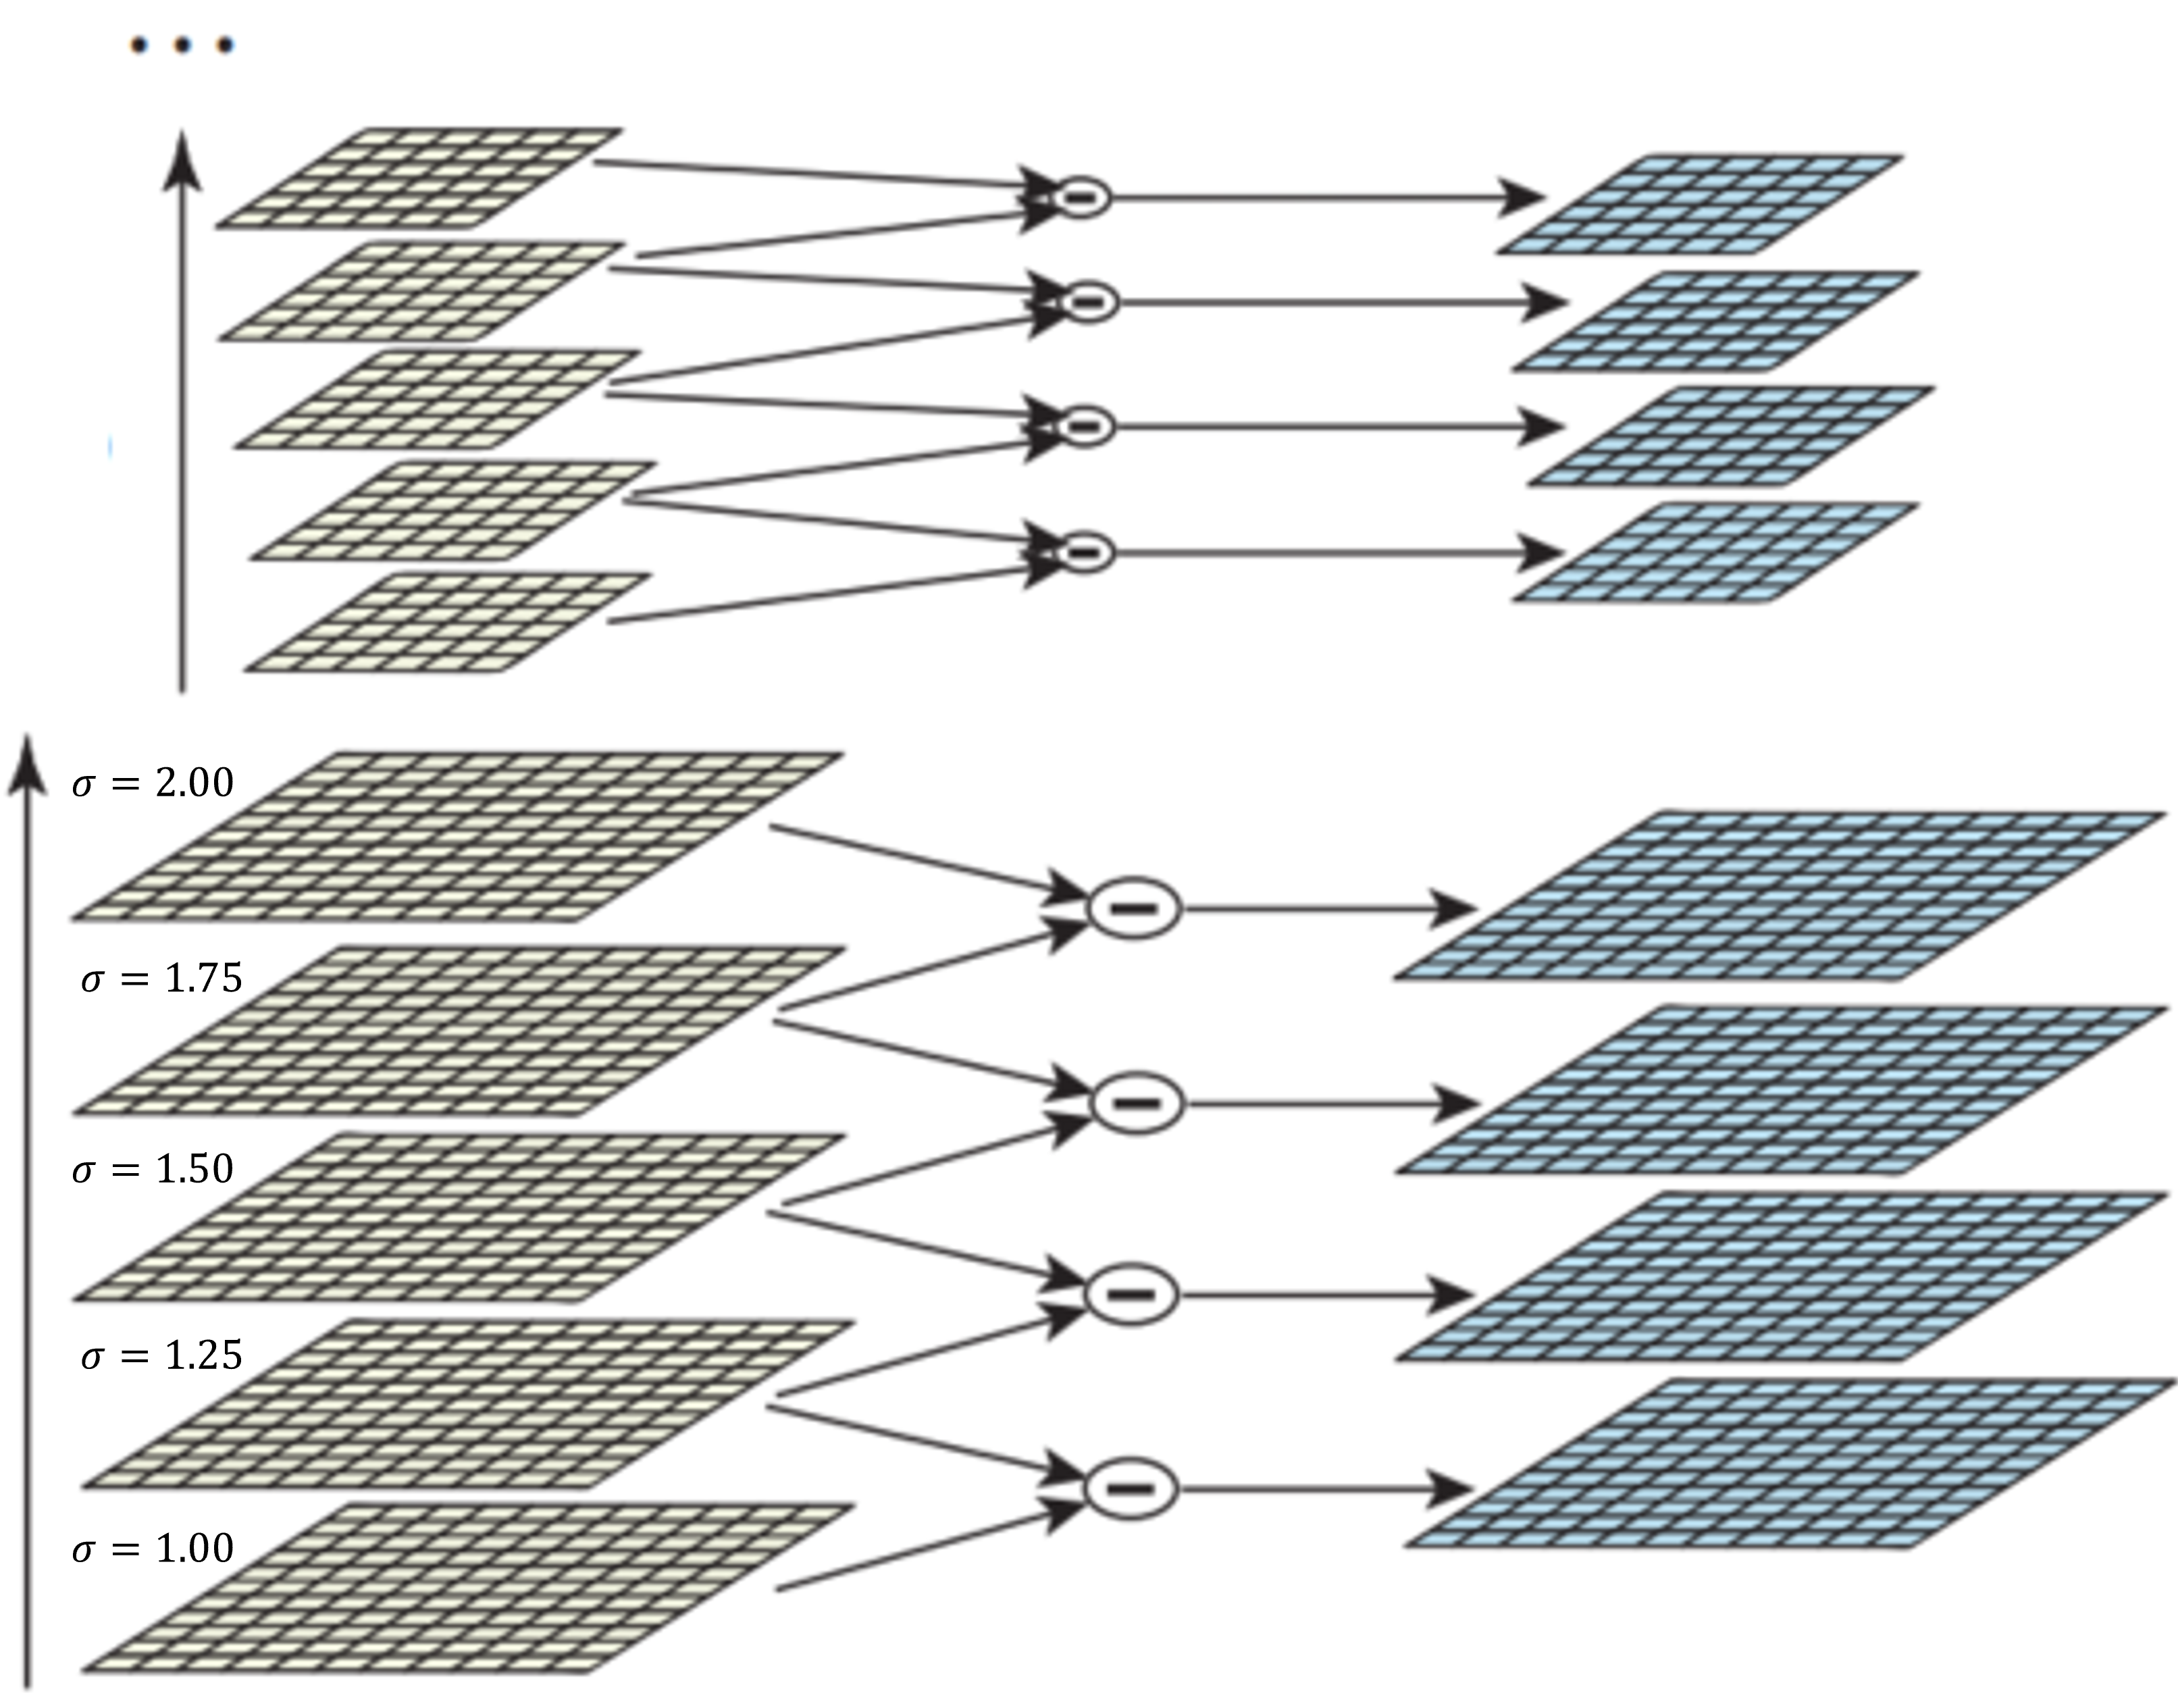
\includegraphics[width=0.6\linewidth]{oktaf.png}
	\caption{Oktaf pada proses konvolusi SIFT}
	\label{fig:oktaf}
\end{figure}

\subsection{Penentuan Orientasi}
Untuk dapat invarian terhadap rotasi gambar, setiap \textit{keypoint} perlu memiliki orientasi yang konsisten. Untuk mendapatkan orientasi yang sama pada setiap rotasi gambar, orientasi perlu ditentukan dari atribut yang akan selalu sama bagaimanapun gambar dirotasi. Untuk itu orientasi \textit{keypoint} ditentukan dengan menggunakan orientasi yang dominan dari \textit{pixel-pixel} di sekitar \textit{keypoint}. Luas daerah yang digunakan untuk mendapat orientasi ditentukan oleh skala dari \textit{keypoint}. 

Penentuan orientasi yang dominan dihitung dengan menggunakan \textit{magnitude}, $m(x,y)$, dan orientasi, $\theta(x,y)$, dari \textit{pixel-pixel} dengan menggunakan rumus berikut, $L(x,y)$ merupakan gambar hasil konvolusi:
\begin{equation}
	\label{eq:magnitude}
	m(x,y)=\sqrt{(L(x+1,y)-L(x-1,y))^{2}+L(x,y+1)-L(x,y+1))^{2}}
\end{equation}
\begin{equation}
	\label{eq:orientasi}
	\theta(x,y)=\tan^{-1}((L(x,y+1)-L(x,y-1))/(L(x+1,y)-L(x-1,y)))
\end{equation}
Setiap \textit{pixel} akan dihitung orientasi dan \textit{magnitude}-nya. \textit{Magnitude} akan digunakan sebagai bobot dari \textit{pixel} tersebut. Selain \textit{magnitude}, bobot sebuah \textit{pixel} juga dipengaruhi oleh \textit{Gaussian Weighting}. \textit{Pixel} yang posisinya dekat dengan titik pusat (pusat \textit{keypoint}) akan memiliki bobot yang lebih tinggi dibanding yang lokasinya jauh. Ilustrasi pada Gambar~\ref{fig:gaussian_weighting} menunjukkan bagaimana pembobotan dihitung, \textit{pixel-pixel} yang berada dekat dengan \textit{keypoint} (titik tengah) akan diberi bobot yang lebih besar---ditandai dengan lingkaran yang tebal. Sedangkan bobot akan semakin berkurang untuk \textit{pixel} yang jauh dari \textit{keypoint}.
\begin{figure}[H]
	\centering
	\includegraphics[width=0.45\linewidth]{gaussian_weighting.png}
	\caption{Ilustrasi pembobotan pada \textit{Gaussian Weighting}. Titik tengah merupakan \textit{keypoint} yang diperiksa sedangkan setiap kotak merupakan \textit{pixel-pixel} di sekitar \textit{keypoint}. Tanda panah pada tiap kotak menunjukkan \textit{magnitude} dan orientasi \textit{pixel} tersebut, panjang panah merupakan nilai \textit{magnitude} dan arahnya merupakan orientasi}
	\label{fig:gaussian_weighting}
\end{figure} 

Setelah setiap \textit{pixel} sudah dihitung orientasi dan bobotnya---menggunakan \textit{magnitude} dan \textit{Gaussian Weighting}---nilai bobot tersebut akan dimasukkan ke dalam histogram berdasarkan orientasinya. Histogram yang digunakan memiliki 36 bin yang masing-masing mewakili 10 derajat orientasi. Ilustrasi dapat dilihat pada Gambar~\ref{fig:hist_orientasi}.
\begin{figure}[H]
	\centering
	\includegraphics[width=0.8\linewidth]{hist_orientasi.png}
	\caption{Histogram untuk menentukan orientasi dari \textit{keypoint}. Bin dengan nilai tertinggi (tanda panah biru) akan digunakan sebagai orientasi dari \textit{keypoint}. Untuk bin lain yang jumlahnya berada dalam rentang $80\%$ dari bin tertinggi (tanda panah hijau) digunakan untuk membuat \textit{keypoint baru}.}
	\label{fig:hist_orientasi}
\end{figure}

Dari histogram tersebut puncak nilai bin tertinggi akan digunakan sebagai orientasi dari \textit{keypoint}. Untuk puncak-puncak lain yang berada dalam rentang $80\%$ dari puncak tertinggi akan digunakan untuk membuat \textit{keypoint} baru pada lokasi yang sama dengan orientasi yang berbeda sesuai dengan nilai orientasi pada bin tersebut.

\subsection{Pembuatan Deskriptor}
Setelah didapatkan \textit{keypoint} beserta skala dan orientasinya, perlu untuk diberikan sebuah identitas pada setiap \textit{keypoint}. Pemberian identitas ini berguna untuk mengidentifikasi \textit{keypoint} yang satu dengan yang lainnya, agar dapat ditemukan \textit{keypoint-keypoint} dengan ciri yang sama. Identifikasi \textit{keypoint} ditentukan dengan membuat sebuah vektor deskriptor, yaitu vektor yang mendeskripsikan daerah di sekitar \textit{keypoint}. Vektor deskriptor pada SIFT berbentuk vektor sepanjang 128 bilangan bulat.

Pembuatan vektor dilakukan dengan mengambil daerah di sekitar \textit{keypoint} dari gambar yang terlebih dahulu dirotasi sesuai dengan orientasi \textit{keypoint}, ukuran daerah berdasarkan pada skala. Daerah tersebut kemudian dibagi menjadi $4\times4$ subdaerah. Untuk setiap subdaerah dihitung nilai \textit{magnitude} dan orientasi setiap \textit{pixel}-nya dengan diberi bobot menggunakan \textit{Gaussian Weighting} lalu hasilnya dimasukkan ke dalam histogram dengan 8 bin. Setiap bin dalam histogram mewakili 45 derajat orientasi, jumlah dari setiap bin ini akan dijadikan nilai pada vektor deskriptor. Teradapat total 16 subdaerah dengan setiap daerah menghasilkan 8 bilangan, sehingga didapat total sebanyak $16\times8=128$ elemen untuk vektor deskriptor. 

\section{ORB (Oriented FAST and Rotated BRIEF)}
\label{sec:orb}
ORB adalah metode pencarian fitur lokal yang dijelaskan pada~\cite{rublee2011orb}. ORB dapat menemukan fitur lokal dengan lebih cepat jika dibandingkan dengan SIFT, walaupun fitur lokal yang dihasilkan tidak seakurat yang dihasilkan SIFT. ORB mencari fitur lokal dengan mencari \textit{pixel} yang merupakan \textit{keypoint}. \textit{Keypoint} dalam ORB dicari dengan ide bahwa sebuah \textit{pixel} yang merupakan sudut akan memiliki daerah kontinu dengan nilai intensitas yang lebih kecil atau lebih besar dari nilai intensitas \textit{pixel} tersebut. Fitur lokal yang dihasilkan ORB akan memiliki sebuah vektor deskriptor yang berbentuk vektor biner sebanyak 256 elemen. Tahap pencarian fitur lokal pada ORB dibagi menjadi 4 langkah yang dijelaskan pada subbab-subbab berikut.

\subsection{Pencarian Keypoint}
Untuk menentukan apakah sebuah \textit{pixel} dalam gambar merupakan \textit{keypoint}, ORB mengambil nilai \textit{pixel} tersebut dan 16 \textit{pixel} di sekitarnya yang membentuk lingkaran. Dari ke 16 \textit{pixel} tersebut dibandingkan nilainya dengan \textit{pixel} yang di tengah $p$, yaitu \textit{pixel} yang ingin diperiksa apakah merupakan \textit{keypoint}. Sebuah \textit{pixel} merupakan \textit{keypoint} jika dari 16 \textit{pixel} di sekitarnya terdapat setidaknya $n$ \textit{pixel} kontinu yang nilainya lebih besar dari nilai $p + t$ atau lebih kecil dari $p - t$. Proses ini diilustrasikan pada Gambar~\ref{fig:orb_keypoint}

\begin{figure}[H]
	\centering
	\includegraphics[width=0.5\linewidth]{orb_keypoint.png}
	\caption{Ilustrasi \textit{keypoint} pada ORB. Titik tengah pada gambar tersebut memiliki \textit{pixel-pixel} dengan nilai jauh lebih kecil (lebih gelap) yang mengelilinginya. \textit{Pixel-pixel} yang mengelilingi tersebut seakan membentuk sudut dengan titik tengah sebagai pusatnya.}
	\label{fig:orb_keypoint}	
\end{figure}

\subsection{Penentuan Skala}
\textit{Keypoint} yang telah dideteksi pada tahap awal perlu untuk dapat terdeteksi juga walaupun ukuran gambar berubah agar sifatnya invarian terhadap skala. Untuk mencapai sifat ini ORB menggunakan metode \textit{Image Pyramid}. ORB menggunakan \textit{Image Pyramid} dengan cara memperkecil ukuran gambar beberapa kali dan untuk setiap ukuran gambar dilakukan deteksi untuk \textit{keypoint}. 

Ilustrasi dapat dilihat pada Gambar~\ref{fig:orb_pyramid}. Pada ilustrasi tersebut gambar awal diperkecil beberapa kali dengan membagi panjang dan lebarnya menjadi setengahnya. Untuk setiap ukuran gambar dicari \textit{keypoint-keypoint}-nya.

\begin{figure}[H]
	\centering
	\includegraphics[width=0.5\linewidth]{orb_pyramid.png}
	\caption{\textit{Image Pyramid} pada ORB}
	\label{fig:orb_pyramid}	
\end{figure}

\section{BSIS (Best Score Increasing Subsequence)}
\label{sec:bsis}
Pada tahapan OIR (lihat~\ref{sec:oir}) sebuah pasangan fitur lokal perlu untuk memiliki sifat yang mirip (dilihat dari vektor deskriptornya) dan juga konsisten secara geometris. Pasangan yang konsisten secara geometris adalah pasangan yang memiliki posisi spasial yang konsisten terhadap objek (fitur lokal) di sekitarnya. Salah satu metode yang dapat digunakan untuk menentukan apakah pasangan fitur lokal bersifat konsisten secara geometris adalah BSIS.
 
\section{KD-Tree}
\label{sec:kdtree}


\section{Clustering}
\label{sec:clustering}

\subsection{Agglomerative}
\label{subsec:agglomerative}

\subsection{DBSCAN}
\label{subsec:dbscan}
